% !TeX root = ../thesis.tex

\section{Software Development Life Cycle}\label{sec:se-sdlc}
An implementation of the SDLC consists of two major components. First, the process is broken down into several smaller phases. Depending on the nature of the software, it is possible to omit steps or add more steps. I have compiled a simple yet generic approach from multiple sources \cite{2010govardhan, 7106435}, to which most software projects adhere. This approach consists of five phases.
\begin{enumerate}
	\bolditem{Requirements phase} This is the initial phase of the development process. During this phase, the developer gets acquainted with the project and compiles a list of the desired functionalities \cite{7106435}. Using this information, the developer eventually decides on the required hardware specifications and possible external software which will need to be acquired.
	
	\bolditem{Design phase} After the developer has gained sufficient knowledge about the project requirements, they can use this information to draw an architectural design of the application. This design consists of multiple documents, including user stories and UML-diagrams.
	
	\bolditem{Implementation phase} During this phase, the developer will write code according to the specifications defined in the architectural designs.
	
	\bolditem{Testing phase} This is the most important phase. During this phase, the implementation is tested to identify potential bugs before the application is used by other users.
	
	\bolditem{Operational phase} In the final phase, the project is fully completed and it is integrated in the existing business environment.
\end{enumerate}

\noindent Subsequently, a model is chosen to define how to transition from one phase into another phase. A manifold of models exist \cite{2010govardhan}, each having advantages and disadvantages, but I will consider the basic yet most widely used model, which is the Waterfall model by Benington \cite{united1956symposium}. The initial Waterfall model required every phase to be executed sequentially and in order, cascading. However, this imposes several issues, the most prevalent being the inability to revise design decisions taken in the second phase, when performing the actual implementation in the third phase. To mitigate this, an improved version of the Waterfall model was proposed by Royce \cite{Royce:1987:MDL:41765.41801}. This version allows a phase to transition back to a previous phase (\autoref{fig:waterfall-royce}).

\begin{figure}[htbp!]
	\centering
	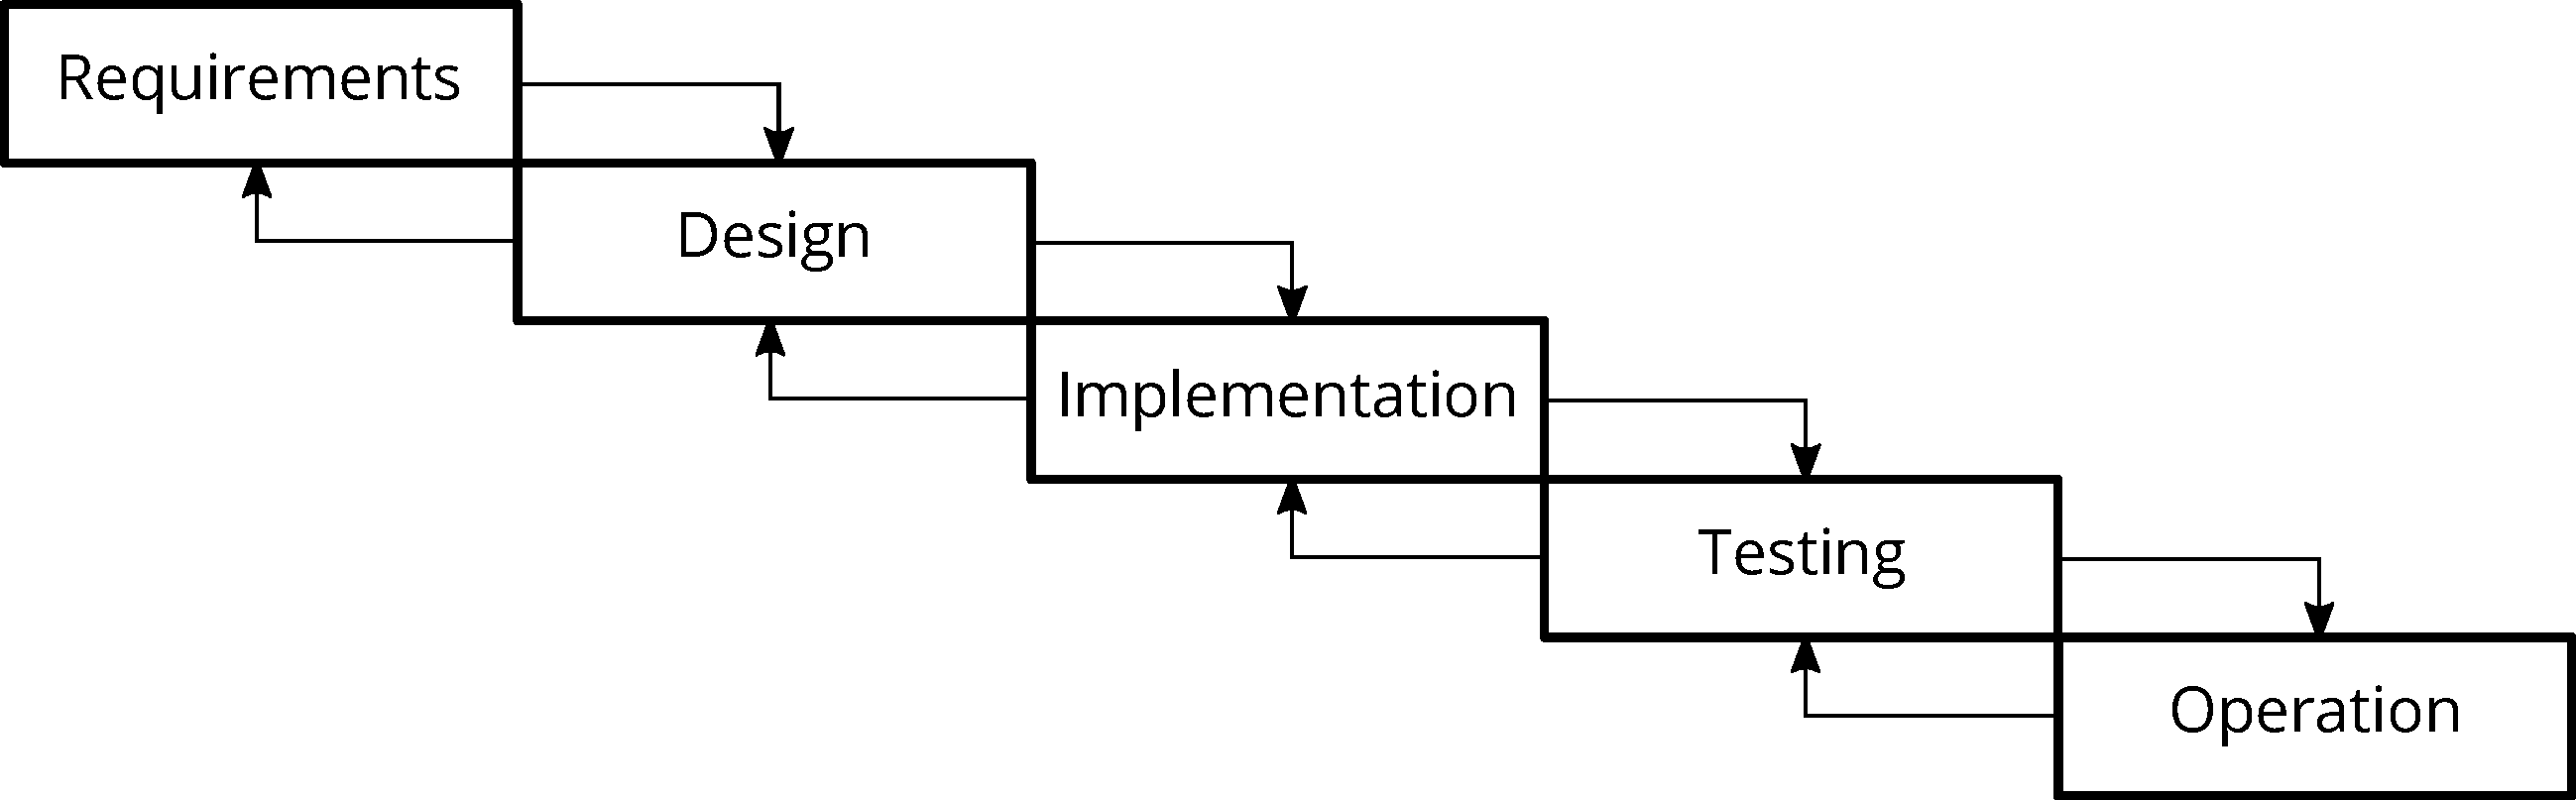
\includegraphics[width=\textwidth]{assets/sdlc.pdf}
	\caption{Improved Waterfall model by Royce}
	\label{fig:waterfall-royce}
\end{figure}

\noindent In this thesis I will solely focus on the implementation and testing phase, as these are the most time-consuming phases of the entire process. The modification to the Waterfall model by Royce is particularly useful when applied to these two phases, in the context of \emph{software regressions}. A regression \cite{10.1007/978-3-540-77966-7_18} is a feature that was previously working correctly, but is now malfunctioning. This behaviour can have external causes, such as a change in the system clock because of daylight saving time, but can also be the result of a change to another, seemingly unrelated part of the application code \cite{6588537}.\\

\noindent Software regressions and other functional bugs can ultimately incur disastrous effects, such as severe financial loss or damage to the reputation of the software company. The most famous example in history is without any doubt the explosion of the Ariane 5-rocket, which was caused by an integer overflow \cite{581900}. In order to reduce the risk of bugs, malfunctioning components should be detected as soon as possible to proactively defend against potential failures. Because of this reason, the testing phase is to be considered as the most important phase of the entire development process and an application should therefore include sufficient tests. The collection of all tests included in an application, or a smaller chosen subset of certain tests, is referred to as the \emph{test suite}. Tests can be classified in multiple categories, this thesis will consider three distinguishable categories:

\begin{enumerate}
	\bolditem{Unit test} This is the most basic kind of test. The purpose of a unit test is to verify the behaviour of an individual component \cite{whittaker2000}. The scope of a unit test should be limited to a small and isolated piece of code, such as one function. Unit tests are typically implemented as \emph{white-box tests} \cite[p.~12]{6588537}. A white-box test is constructed by manually inspecting the function under test, to identify important \emph{edge values}. The unit test should then feed these values as arguments to the function under test, to observe its behaviour. Common edge cases include zero, negative numbers, empty arrays or array boundaries that might result in an overflow.
	
	\bolditem{Integration test} A more advanced test, an integration test verifies the interaction between multiple individually tested components \cite{whittaker2000}. Examples of integration tests include the communication between the front-end and the back-end side of an application. As opposed to unit tests, an integration test is an example of a \emph{black-box} test \cite[p.~6]{6588537}, meaning that implementation-specific details should be irrelevant or unknown when writing an integration test.
	
	\bolditem{Regression test} After a regression has been detected, a regression test \cite[p.~372]{8016712} is added to the test suite. This regression test should replicate the exact conditions and sequence of actions that have caused the regression, to warden the implementation against subsequent failures if the same conditions would reapply in the future.
\end{enumerate}

% !TeX root = ../thesis.tex

\section{Test Suite Assessment}

\subsection{Coverage}
The most frequently used metric to measure the quantity and thoroughness of a test suite is the \emph{code coverage} or \emph{test coverage} \cite[p.~467]{8016712}. The test coverage indicates which fraction of the application code is hit by at least one test case in the test suite. Internally, a coverage framework calculates the coverage ratio by augmenting every application statement using binary instrumentation. A hook is inserted before and after every statement to detect which statements are executed by the test cases. Many different criteria exist to interpret these results and thus to express the fraction of covered code \cite{Myers:2011:AST:2161638}. The two most commonly used criteria are \emph{statement coverage} and \emph{branch coverage}.

\paragraph*{Statement coverage} Statement coverage expresses the fraction of statements that are executed by any test case in the test suite, over the total amount of statements in the code \cite{6588537}. Similarly, we can calculate the \emph{line coverage} as the fraction of covered code lines. Since one statement can span multiple lines and one line may also contain more than one statement, both of these criteria are intrinsically related. Statement coverage is heavily criticised in literature \cite[p.~37]{Myers:2011:AST:2161638} since it is possible to achieve a statement coverage percentage of $\SI{100}{\percent}$ on code of which we can prove it is malfunctioning. Consider \cref{lst:statement-coverage-fail}. If a test case would call the example-function with arguments $\{a = 1, b = 2\}$, then the test case will pass, and every statement will be covered, resulting in a statement coverage of $\SI{100}{\percent}$. However, suppose we would call the function with arguments $\{a = 0, b = 0\}$. The first argument matches the first condition of the branch but will trigger a \texttt{division-by-zero} error, even though the previous combination of arguments reported a complete statement coverage. This simple example was already sufficient to illustrate that statement coverage is not trustworthy. However, statement coverage may still prove useful for other purposes, such as detecting unreachable code which we may safely remove.

\begin{lstlisting}[caption=Example of irrelevant statement coverage in C.,label=lst:statement-coverage-fail,language=C]
	int example(int a, int b) {
 if (a == 0 || b != 0) {
  return a / b;
 }
	}
\end{lstlisting}

\paragraph*{Branch coverage} requires that the test cases traverse every branch of a conditional statement at least once  \cite[p.~37]{Myers:2011:AST:2161638}. For an \texttt{if}-statement, we require two test cases, one for every possible outcome of the condition (\texttt{true} or \texttt{false}). For a loop-statement, we require at least two test cases as well. One test case should never execute the loop, and the other test case should execute every iteration. Optionally, we can add additional test cases for specific iterations. Observe that, while this criterion is stronger than statement coverage, it will still not detect the bug in \Cref{lst:statement-coverage-fail}. In order to mitigate this, we can use \emph{multiple-condition coverage} \cite[p.~40]{Myers:2011:AST:2161638}. This criterion requires that for every conditional expression, every possible combination of subexpressions is evaluated at least once. If we apply this requirement to \Cref{lst:statement-coverage-fail}, the \texttt{if}-statement will only be covered if we test the following four cases.

\begin{itemize}
	\item $a = 0, b = 0$
	\item $a = 0, b \neq 0$
	\item $a \neq 0, b = 0$
	\item $a \neq 0, b \neq 0$
\end{itemize}

\noindent It should be self-evident that achieving and maintaining a coverage percentage of $\SI{100}{\percent}$ at all times is critical. However, this does not necessarily imply that every line of code, every statement or every branch must be explicitly covered \cite{dein_2019}. Some parts of the code might be irrelevant or untestable, such as wrapper or delegation methods that only call a library function. All major programming languages have frameworks and libraries that enable the collection of coverage information during test execution, and each of these frameworks allows the exclusion parts of the code from the final coverage calculation. As of today, the most popular options are JaCoCo\footnote{\url{https://www.jacoco.org/jacoco/}} for Java, coverage.py\footnote{\url{https://github.com/nedbat/coveragepy}} for Python and simplecov\footnote{\url{https://github.com/colszowka/simplecov}} for Ruby. These frameworks report in-depth statistics on the covered code and indicate which parts require more extensive testing, as illustrated in \Cref{fig:coverage-statistics}.

\subsection{Mutation testing}\label{sssec:mutation-testing}
The previous section has explained how we can identify which parts of the code require additional test cases. However, we cannot yet measure the quality and resilience of the test suite nor its ability to detect future failures. To accomplish this, we can employ \emph{mutation testing}. This technique creates several \emph{mutants} of the application under test. A mutant is a syntactically different instance of the source code. We can create a mutant by applying one or more \emph{mutation operators} to the original source code. These mutation operators attempt to simulate typical mistakes that developers tend to make, such as the introduction of off-by-one errors, removal of statements and the replacement of logical connectors \cite{Offutt2001}. The \emph{mutation order} refers to the amount of mutation operators that have been applied consecutively to an instance of the code. This order is traditionally rather low, as a result of the \emph{Competent Programmer Hypothesis}, which states that programmers develop programs which are near-correct \cite{5487526}.

\paragraph*{Creating and evaluating} the mutant versions of the code is a computationally expensive process which typically requires human intervention. As a result, very few software developers have managed to employ this technique in practice. \Cref{fig:mutation-testing} illustrates the process of applying mutation testing. The first step is to consider the original program $P$ and a set of test cases $TS$, to which we apply mutation operators to construct a broad set of mutants $P'$. Next, we evaluate every test case $t \in TS$ on the original program $P$ to determine the correct behaviour. Note that this step assumes that if the original source code passes the test cases, it is correct. This assumption will only be valid if the test suite contains sufficient thorough unit tests. If at least one of these test cases fails, we have found a bug which we must first resolve before continuing with the mutation analysis. When $P$ successfully passes every test case, we evaluate every test case for each of the mutants. A mutant $p'$ is said to be ``killed'' if its outcome is different from $P$ for at least one test case. Otherwise, we refer to the mutant as ``surviving''. After we have finished executing the test cases on every mutant, we analyse the set of surviving mutants. Every mutant that managed to survive implies a change in the source code that did not trigger any failure in the test cases. As a result, we need to introduce subsequent test cases until we have killed every mutant. However, it is also possible that the surviving mutants are functionally equivalent to $P$ and are, therefore, correct. Since the detection of program equivalence is an impossible problem, we need to verify this manually \cite{5487526, Offutt2001}. Finally, note that although we can use mutation testing to estimate the adequacy of the test suite, it is not flawless, as several mutation operators can cancel each other out \cite{evaluationoftestsuiteminimization}.

\begin{figure}[htbp!]
	\centering
	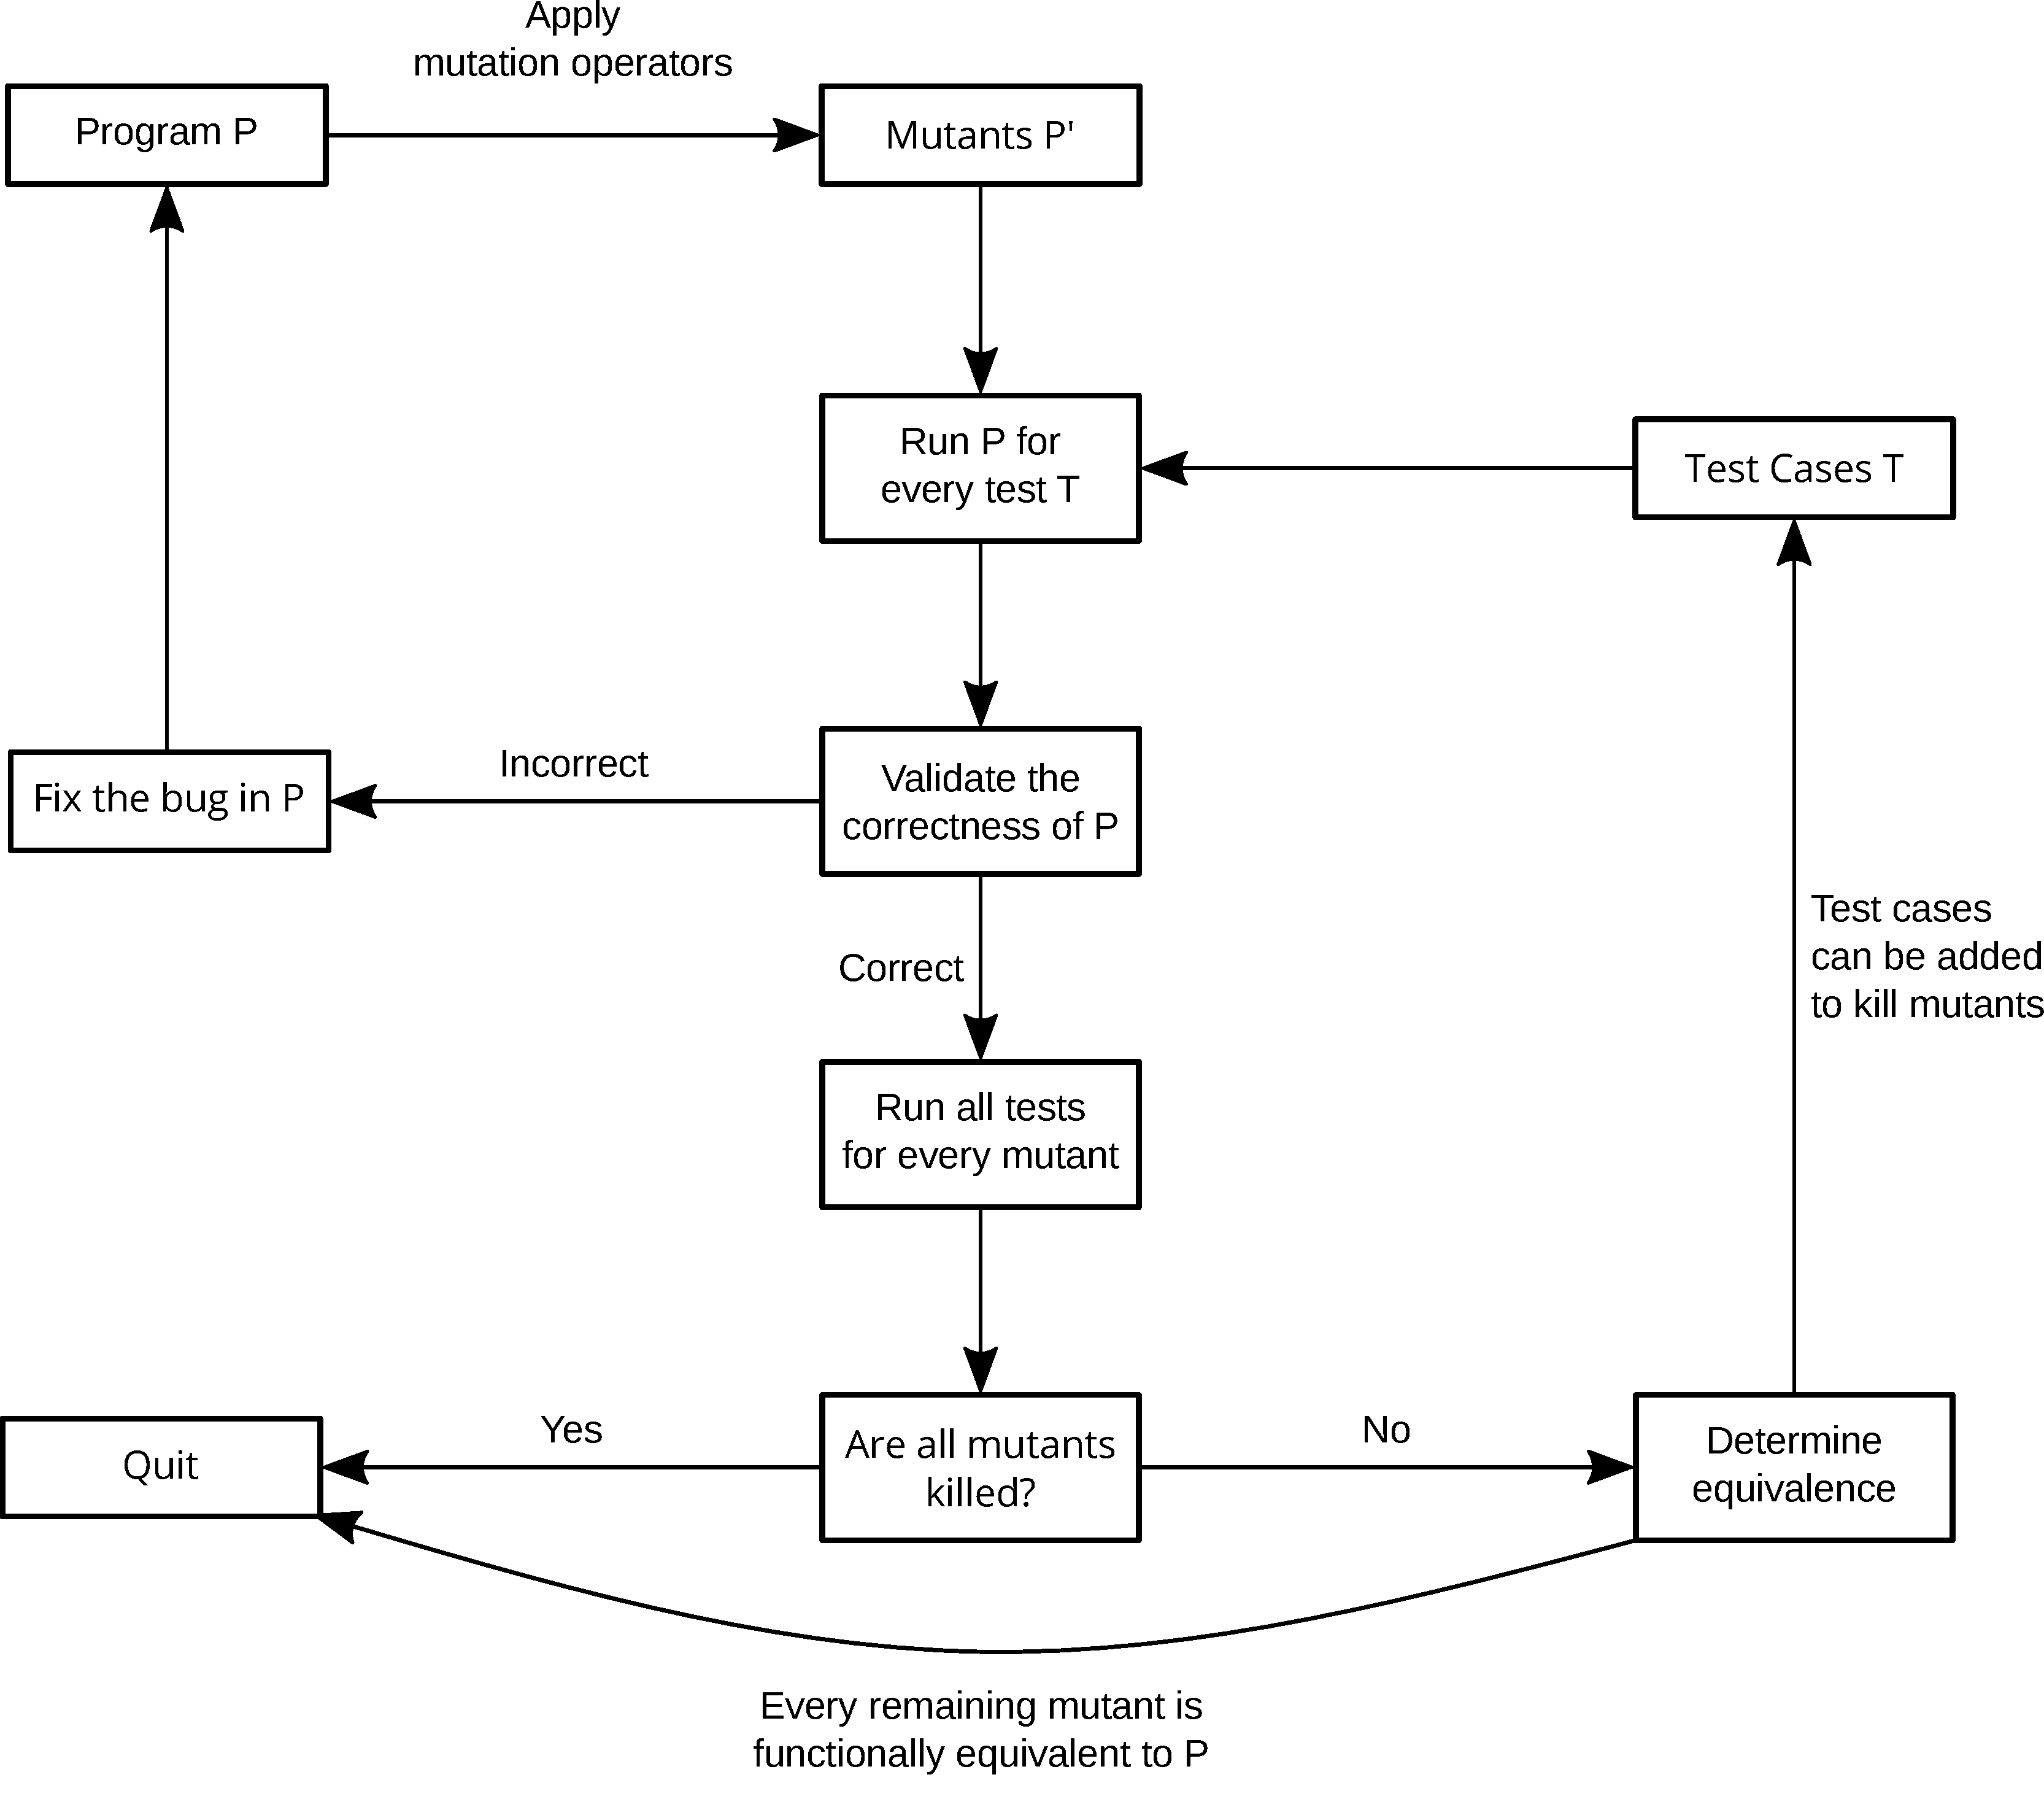
\includegraphics[width=\textwidth]{assets/images/mutation-testing.pdf}
	\caption{Process of Mutation Testing (based on \cite{Offutt2001})}
	\label{fig:mutation-testing}
\end{figure}

\noindent After every mutant has either been killed or marked equivalent to the original problem, we can calculate the \emph{mutation score} of the test suite using \cref{eq:mutant-score}. In an adequate test suite, this score is equal to $\SI{1}{}$, which indicates that the test suite was able to detect every mutant instantly.

\begin{equation}\label{eq:mutant-score}
	\text{Mutant Score} = \frac{\text{killed mutants}}{\text{non-equivalent mutants}}
\end{equation}

\begin{figure}[htbp!]
	\centering
	\subfloat[JaCoCo coverage report of \url{https://github.com/thepieterdc/dodona-api-java}]{%
		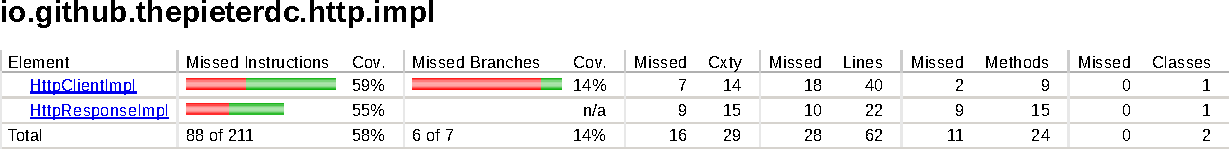
\includegraphics[clip,width=\textwidth]{assets/images/coverage-jacoco.pdf}
	}
	\newline
	\subfloat[coverage.py report of \url{https://github.com/codecov/example-python}]{%
		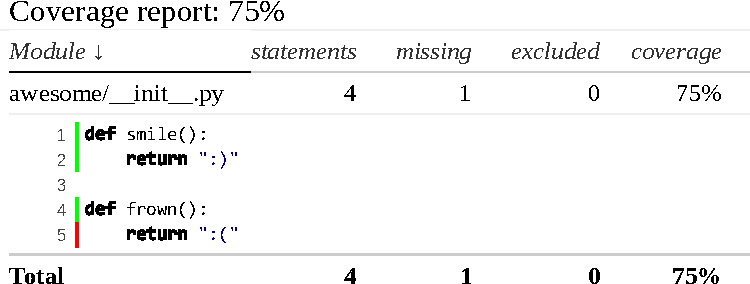
\includegraphics[clip,width=\textwidth]{assets/images/coverage-coveragepy.pdf}
	}
	\newline
	\subfloat[simplecov report of \url{https://github.com/dodona-edu/dodona}]{%
		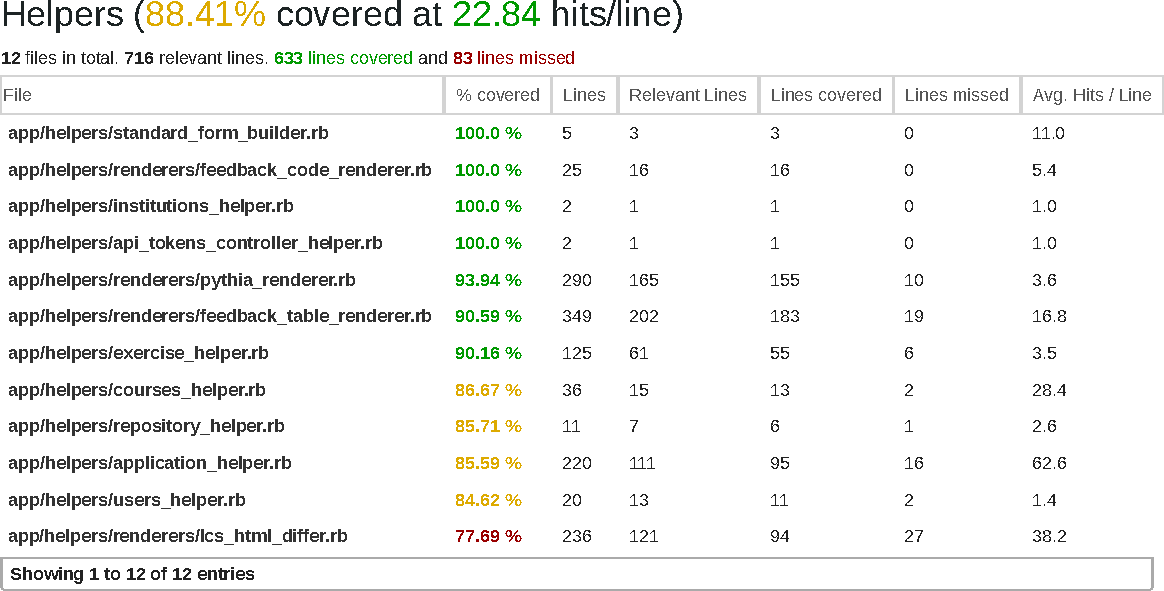
\includegraphics[clip,width=\textwidth]{assets/images/coverage-simplecov.pdf}
	}
	\caption{Statistics from Code coverage tools}
	\label{fig:coverage-statistics}
\end{figure}